% Formal vector figures for the JCIIOT technical report.
% These macros replace the Markdown/ASCII diagrams and raster-only charts.

\newcommand{\SystemArchitectureFigure}{%
\begin{figure}[htbp]
  \centering
  \resizebox{\linewidth}{!}{%
  \begin{tikzpicture}[
    >=Latex,
    stage/.style={
      draw=ReportNavy,
      line width=0.65pt,
      rounded corners=1.2mm,
      minimum width=27.8mm,
      minimum height=16mm,
      text width=24.8mm,
      align=center,
      font=\sffamily\bfseries\scriptsize,
      text=ReportInk,
      blur shadow={shadow opacity=0.10,shadow yshift=-0.6mm}
    },
    flow/.style={-Latex,line width=1.05pt,draw=ReportBlue},
    note/.style={font=\sffamily\scriptsize,text=ReportMuted,align=center}
  ]
    \node[stage,fill=ReportPaleBlue] (task) {Official task\\identifiers};
    \node[stage,fill=ReportPaleTeal,right=4.1mm of task] (plan) {Semantic plan\\+ A* route};
    \node[stage,fill=ReportPaleOrange,right=4.1mm of plan] (motion) {Bounded motion\\+ physical grasp};
    \node[stage,fill=ReportPurple!12,right=4.1mm of motion] (state) {MuJoCo state\\per physics step};
    \node[stage,fill=ReportPaleBlue,right=4.1mm of state] (verify) {Score + audit\\+ full video};

    \draw[flow] (task) -- (plan);
    \draw[flow] (plan) -- (motion);
    \draw[flow] (motion) -- (state);
    \draw[flow] (state) -- (verify);

    \node[note,above=7.5mm of motion] (context)
      {semantic map + live object geometry + payload-aware clearance};
    \draw[-Latex,draw=ReportTeal,line width=0.8pt] (context) -- (motion);

    \node[
      below=7mm of motion,
      fill=ReportNavy,
      text=white,
      rounded corners=1.2mm,
      inner xsep=5mm,
      inner ysep=2.2mm,
      font=\sffamily\bfseries\scriptsize
    ] (gate) {Release only if maximum score AND realism audit AND video integrity all pass};
    \draw[-Latex,draw=ReportNavy,line width=0.8pt] (verify.south) |- (gate.east);
  \end{tikzpicture}%
  }
  \caption{End-to-end execution and evidence flow. Physical execution and independent verification are joined by a conjunctive release gate.}
  \label{fig:system-architecture}
\end{figure}%
}

\newcommand{\ArchitectureDetailFigure}{%
\begin{figure}[htbp]
  \centering
  \resizebox{\linewidth}{!}{%
  \begin{tikzpicture}[
    x=1cm,y=1cm,
    box/.style={
      draw=ReportNavy,
      line width=0.55pt,
      rounded corners=1mm,
      align=center,
      font=\sffamily\scriptsize,
      text=ReportInk,
      minimum height=0.78cm
    },
    lane/.style={font=\sffamily\bfseries\tiny,text=ReportNavy,anchor=east},
    arr/.style={-Latex,draw=ReportBlue,line width=0.8pt},
    feed/.style={-Latex,draw=ReportTeal,line width=0.72pt}
  ]
    \fill[ReportMist,rounded corners=1.5mm] (-0.3,0.15) rectangle (15.2,1.35);
    \fill[ReportMist!65,rounded corners=1.5mm] (-0.3,-1.55) rectangle (15.2,-0.05);
    \fill[ReportMist,rounded corners=1.5mm] (-0.3,-2.95) rectangle (15.2,-1.75);
    \fill[ReportMist!65,rounded corners=1.5mm] (-0.3,-4.55) rectangle (15.2,-3.15);

    \node[lane] at (1.35,0.75) {SEMANTICS};
    \node[box,fill=ReportPaleBlue,text width=2.7cm] (ids) at (3.1,0.75) {official task identifiers};
    \node[box,fill=ReportPaleTeal,text width=4.2cm] (skills) at (8.0,0.75) {move $\rightarrow$ pick\_up $\rightarrow$ move $\rightarrow$ place\_down};
    \node[box,fill=ReportPaleOrange,text width=2.5cm] (fail) at (12.8,0.75) {named fail-closed boundaries};
    \draw[arr] (ids) -- (skills);
    \draw[arr] (skills) -- (fail);

    \node[lane] at (1.35,-0.80) {GEOMETRY};
    \node[box,fill=ReportPaleBlue,text width=2.55cm] (map) at (3.1,-0.80) {semantic map\\+ occupancy grid};
    \node[box,fill=ReportPaleTeal,text width=2.55cm] (live) at (7.25,-0.80) {live object pose\\+ grasp sites};
    \node[box,fill=ReportPaleOrange,text width=2.75cm] (clear) at (11.65,-0.80) {payload clearance\\+ turn preflight};

    \node[lane] at (1.35,-2.35) {EXECUTION};
    \node[box,fill=ReportPaleOrange,text width=9.6cm,minimum height=0.82cm] (exec) at (8.0,-2.35)
      {bounded base motion + dual-arm OSC + continuous carried-object attachment};
    \draw[feed] (map) -- ($(exec.north west)!0.22!(exec.north east)$);
    \draw[feed] (live) -- (exec.north);
    \draw[feed] (clear) -- ($(exec.north west)!0.78!(exec.north east)$);

    \node[lane] at (1.35,-3.85) {EVIDENCE};
    \node[box,fill=ReportPurple!12,text width=2.5cm] (trajectory) at (3.05,-3.85) {per-step trajectory};
    \node[box,fill=ReportPaleBlue,text width=3.25cm] (checks) at (7.15,-3.85) {objective score + contact audit + video};
    \node[box,fill=ReportNavy,text=white,text width=2.65cm,font=\sffamily\bfseries\scriptsize] (release) at (11.75,-3.85) {accept artifact};
    \draw[arr] (exec.south) |- (trajectory.north);
    \draw[arr] (trajectory) -- (checks);
    \draw[arr] (checks) -- node[above,font=\sffamily\tiny,text=ReportMuted]{all PASS} (release);
  \end{tikzpicture}%
  }
  \caption{Layered control architecture. Semantic decisions are deterministic; geometry is read from the live scene; every physical step enters the evidence pipeline.}
  \label{fig:architecture-detail}
\end{figure}%
}

\newcommand{\StateHandoffFigure}{%
\begin{figure}[htbp]
  \centering
  \resizebox{\linewidth}{!}{%
  \begin{tikzpicture}[
    >=Latex,
    box/.style={
      draw=ReportNavy,
      line width=0.58pt,
      rounded corners=1mm,
      minimum height=13mm,
      text width=31mm,
      align=center,
      font=\sffamily\scriptsize,
      text=ReportInk
    },
    flow/.style={-Latex,draw=ReportBlue,line width=0.85pt},
    commit/.style={-Latex,draw=ReportTeal,line width=0.85pt}
  ]
    \node[box,fill=ReportPaleBlue] (n) {Navigation snapshot \(N\)\\robot + every live object};
    \node[box,fill=ReportPaleTeal,right=6mm of n] (init) {Exact wrapper initialization\\reset hook reapplies \(N\)};
    \node[box,fill=ReportPaleOrange,right=6mm of init] (g) {Stepped physical grasp\\produces state \(G\)};
    \node[box,fill=ReportPurple!12,right=6mm of g] (select) {Ownership-aware commit\\select state source};
    \draw[flow] (n) -- (init);
    \draw[flow] (init) -- (g);
    \draw[flow] (g) -- (select);

    \coordinate (branchcenter) at ($(n.south)!0.5!(select.south)$);
    \node[box,fill=ReportPaleOrange,below=8mm of branchcenter,xshift=-29mm,text width=50mm] (fromg)
      {\textbf{Commit from \(G\)}\\target object + robot state};
    \node[box,fill=ReportPaleBlue,below=8mm of branchcenter,xshift=29mm,text width=50mm] (fromn)
      {\textbf{Preserve from \(N\)}\\all non-target material states};
    \coordinate (split) at ([yshift=-3.5mm]select.south);
    \draw[commit] (select.south) -- (split) -| (fromg.north);
    \draw[commit] (split) -| (fromn.north);

    \node[
      below=8mm of $(fromg.south)!0.5!(fromn.south)$,
      draw=ReportNavy,
      line width=0.65pt,
      fill=ReportPaleTeal,
      text=ReportNavy,
      rounded corners=1.1mm,
      text width=105mm,
      align=center,
      minimum height=13mm,
      inner xsep=4mm,
      inner ysep=2.4mm,
      font=\sffamily\scriptsize
    ] (committed) {\textbf{Committed navigation state \(N'\)}\\continuity preserved across repeated L5 cycles};
    \draw[commit] (fromg.south) -- ++(0,-3.5mm) -| ([xshift=-28mm]committed.north);
    \draw[commit] (fromn.south) -- ++(0,-3.5mm) -| ([xshift=28mm]committed.north);
  \end{tikzpicture}%
  }
  \caption{Transactional handoff between navigation and wrapped grasp environments. Completed placements remain unchanged while the target and robot state are committed from the physical grasp rollout.}
  \label{fig:state-handoff}
\end{figure}%
}

\newcommand{\LFivePlacementFigure}{%
\begin{figure}[htbp]
  \centering
  \begin{tikzpicture}
    \begin{axis}[
      width=0.76\linewidth,
      height=0.57\linewidth,
      axis equal image,
      xmin=-0.90,xmax=0.90,
      ymin=-0.90,ymax=0.90,
      xlabel={X offset from official target center (m)},
      ylabel={Y offset from official target center (m)},
      tick label style={font=\scriptsize},
      label style={font=\sffamily\small,text=ReportInk},
      grid=both,
      major grid style={draw=ReportRule,line width=0.35pt},
      axis line style={draw=ReportNavy,line width=0.55pt},
      legend style={font=\sffamily\scriptsize,draw=none,at={(0.5,-0.18)},anchor=north,legend columns=2},
      clip=false
    ]
      \addplot[domain=0:360,samples=181,ReportOrange,dashed,line width=1.35pt]
        ({0.8*cos(x)},{0.8*sin(x)});
      \addlegendentry{official 0.80 m scoring radius}
      \addplot[only marks,mark=+,mark size=5pt,mark options={line width=1.2pt,ReportNavy}]
        coordinates {(0,0)};
      \addlegendentry{official target center}

      \addplot[only marks,mark=*,mark size=4.7pt,ReportTeal]
        coordinates {(0.0095,0.065156)};
      \addplot[only marks,mark=*,mark size=4.7pt,ReportBlue]
        coordinates {(0.665918,0.047620)};
      \addplot[only marks,mark=*,mark size=4.7pt,ReportOrange]
        coordinates {(-0.645914,0.024040)};
      \node[anchor=south west,font=\sffamily\scriptsize,text=ReportInk] at (axis cs:0.03,0.08) {front: 0.066 m};
      \node[anchor=south west,font=\sffamily\scriptsize,text=ReportInk] at (axis cs:0.57,0.08) {center: 0.668 m};
      \node[anchor=south west,font=\sffamily\scriptsize,text=ReportInk] at (axis cs:-0.62,0.06) {back: 0.646 m};
    \end{axis}
  \end{tikzpicture}
  \caption{Terminal L5 tote positions relative to the official target center. All three physical placements lie within the scoring radius.}
  \label{fig:l5-placement}
\end{figure}%
}

\newcommand{\ContinuityMarginsFigure}{%
\begin{figure}[htbp]
  \centering
  \resizebox{\linewidth}{!}{%
  \begin{tikzpicture}[
    cell/.style={minimum width=25.2mm,minimum height=8.6mm,anchor=center,font=\sffamily\bfseries\scriptsize},
    metric/.style={font=\sffamily\scriptsize,text=ReportNavy,align=center},
    level/.style={font=\sffamily\bfseries\scriptsize,text=ReportNavy}
  ]
    \matrix (heat) [matrix of nodes,ampersand replacement=\&,row sep=0pt,column sep=0pt,nodes={cell},nodes in empty cells] {
      |[fill=ReportBlue!58!white,text=white]| 0.58x \& |[fill=ReportBlue!33!white,text=ReportInk]| 0.33x \& |[fill=ReportBlue!64!white,text=white]| 0.64x \& |[fill=ReportBlue!48!white,text=ReportInk]| 0.48x \& |[fill=ReportBlue!64!white,text=white]| 0.64x \\
      |[fill=ReportBlue!59!white,text=white]| 0.59x \& |[fill=ReportBlue!65!white,text=white]| 0.65x \& |[fill=ReportBlue!64!white,text=white]| 0.64x \& |[fill=ReportBlue!48!white,text=ReportInk]| 0.48x \& |[fill=ReportBlue!26!white,text=ReportInk]| 0.26x \\
      |[fill=ReportBlue!59!white,text=white]| 0.59x \& |[fill=ReportBlue!33!white,text=ReportInk]| 0.33x \& |[fill=ReportBlue!64!white,text=white]| 0.64x \& |[fill=ReportBlue!35!white,text=ReportInk]| 0.35x \& |[fill=ReportBlue!17!white,text=ReportInk]| 0.17x \\
      |[fill=ReportBlue!59!white,text=white]| 0.59x \& |[fill=ReportBlue!66!white,text=white]| 0.66x \& |[fill=ReportOrange!85!white,text=white]| 0.85x \& |[fill=ReportBlue!53!white,text=ReportInk]| 0.53x \& |[fill=ReportBlue!44!white,text=ReportInk]| 0.44x \\
      |[fill=ReportBlue!59!white,text=white]| 0.59x \& |[fill=ReportBlue!34!white,text=ReportInk]| 0.34x \& |[fill=ReportBlue!64!white,text=white]| 0.64x \& |[fill=ReportOrange!86!white,text=white]| 0.86x \& |[fill=ReportBlue!72!white,text=white]| 0.72x \\
    };
    \foreach \row/\name in {1/L1,2/L2,3/L3,4/L4,5/L5}{
      \node[level,left=3mm of heat-\row-1] {\name};
    }
    \node[metric,above=3mm of heat-1-1] {base\\translation};
    \node[metric,above=3mm of heat-1-2] {base\\rotation};
    \node[metric,above=3mm of heat-1-3] {robot joint\\change};
    \node[metric,above=3mm of heat-1-4] {material\\translation};
    \node[metric,above=3mm of heat-1-5] {material\\rotation};
    \draw[ReportRule,line width=0.5pt] (heat.north west) rectangle (heat.south east);
    \node[font=\sffamily\scriptsize,text=ReportMuted,below=4mm of heat]
      {cell value = observed frame-to-frame maximum / audit limit; orange marks the two closest approaches to a limit};
  \end{tikzpicture}%
  }
  \caption{Observed continuity maxima normalized by their strict audit limits. Every value remains below 1.0.}
  \label{fig:continuity-margins}
\end{figure}%
}

\newcommand{\VideoEvidenceFigure}{%
\begin{figure}[htbp]
  \centering
  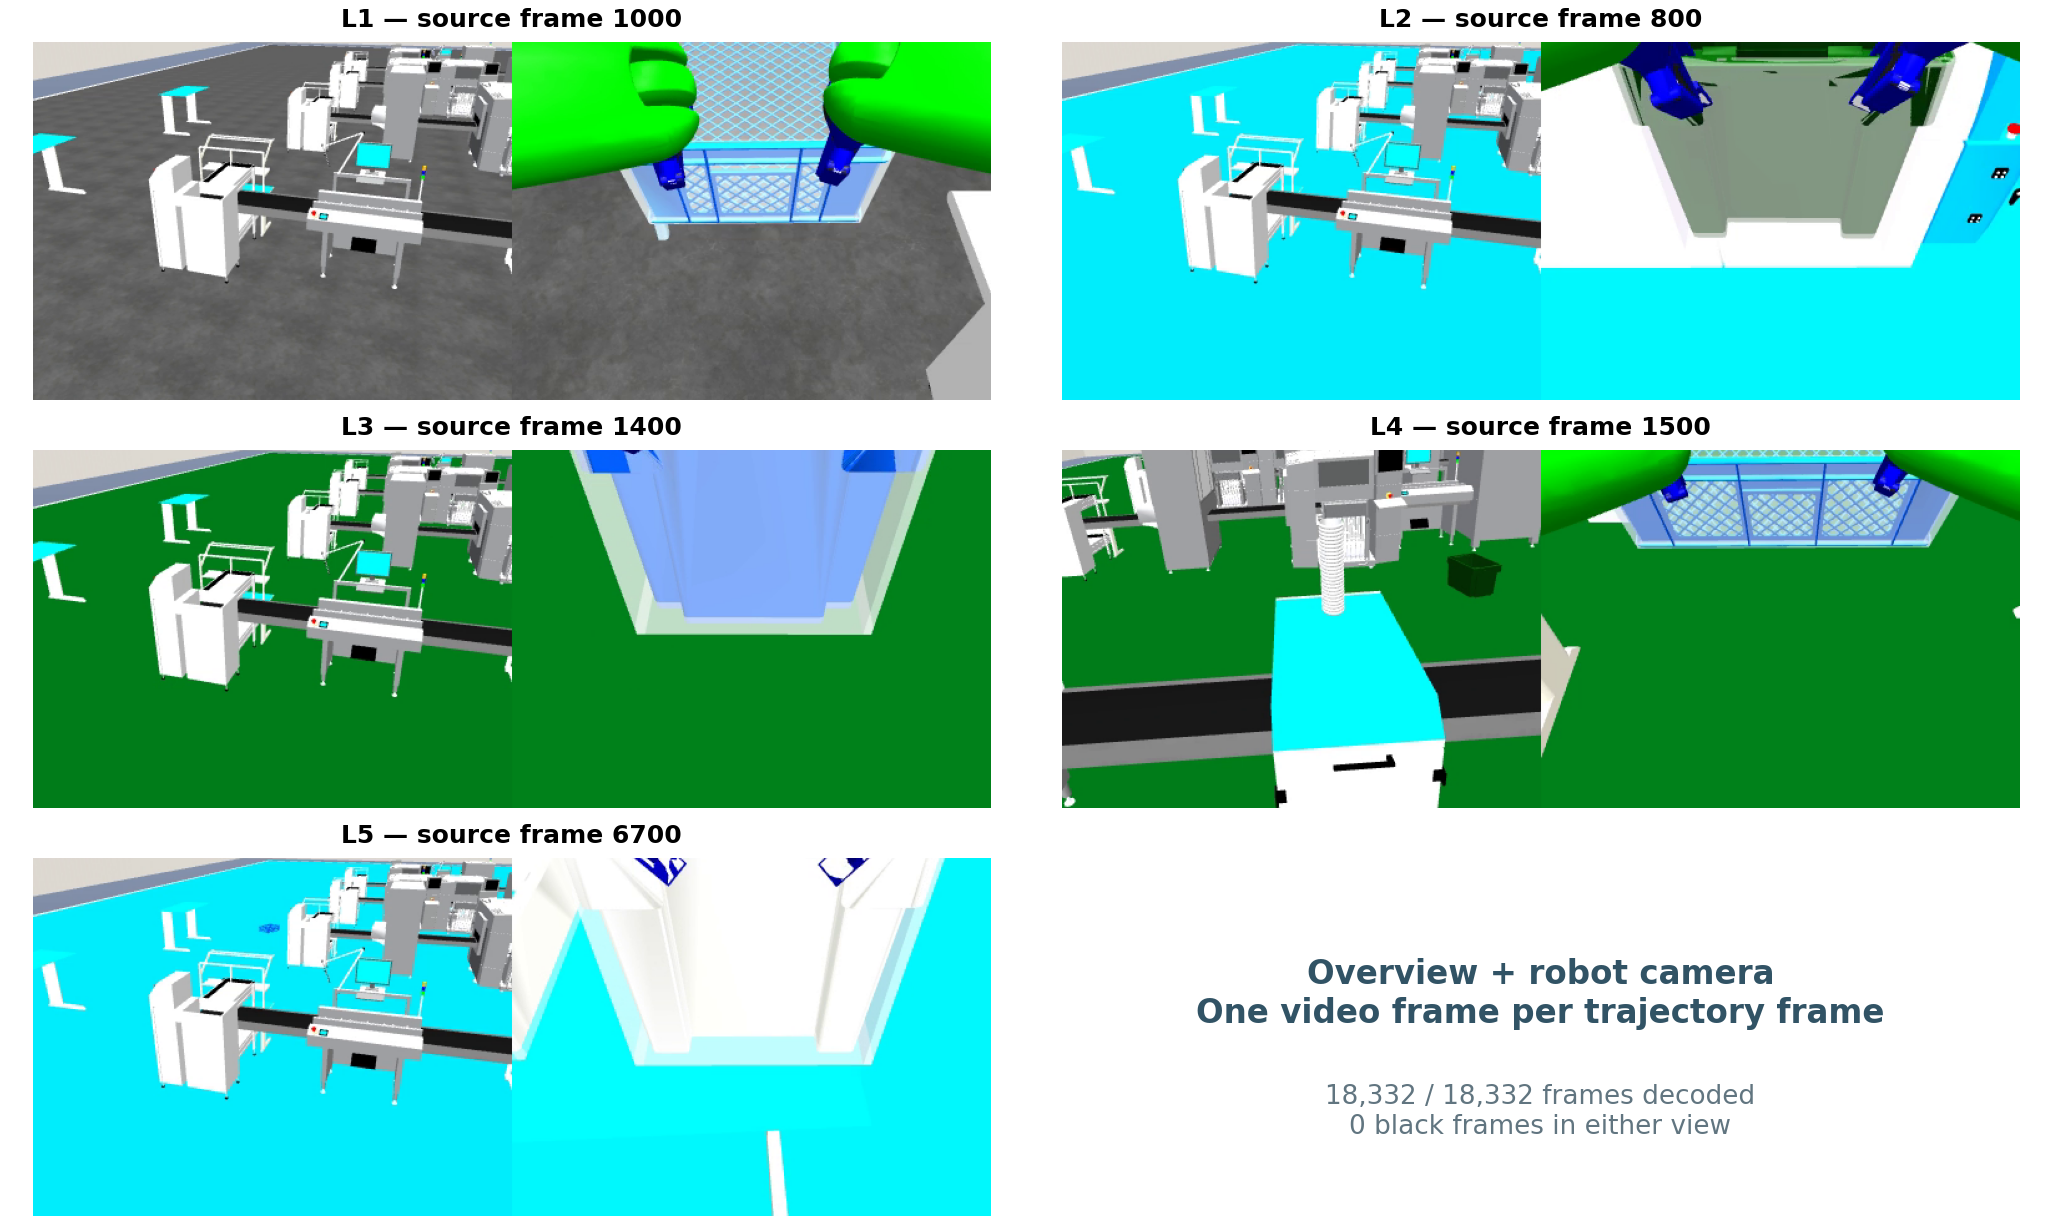
\includegraphics[width=\linewidth]{../assets/video_contact_sheet.png}
  \caption{Representative synchronized overview and robot-camera frames from the L1--L5 full-frame videos. Each encoded video contains one frame per source trajectory state.}
  \label{fig:video-evidence}
\end{figure}%
}
